\subsection{Introduction to the Choicely voting platform}
    % what does the company do? 
    Choicely is a voting platform that... The platform has already hosted numerous contests in various fields, such as beauty pageants, public polls, design contests, sport events among many others. The customer base of the firm consist of mainly Finnish broadcasters, publishers and advertisers. The customer and user base is constantly growing with many international companies from all around the world.
    
    % what are the contests like, what kind of configuration settings are available?
    The contests in the platform are... Users may participate in arbitrary number of contests from three platforms: the two most popular mobile platforms (iOS and Android) and the web interface (Figure \ref{choicely_platforms}). 

    \begin{figure}[h] 
		\begin{center}
			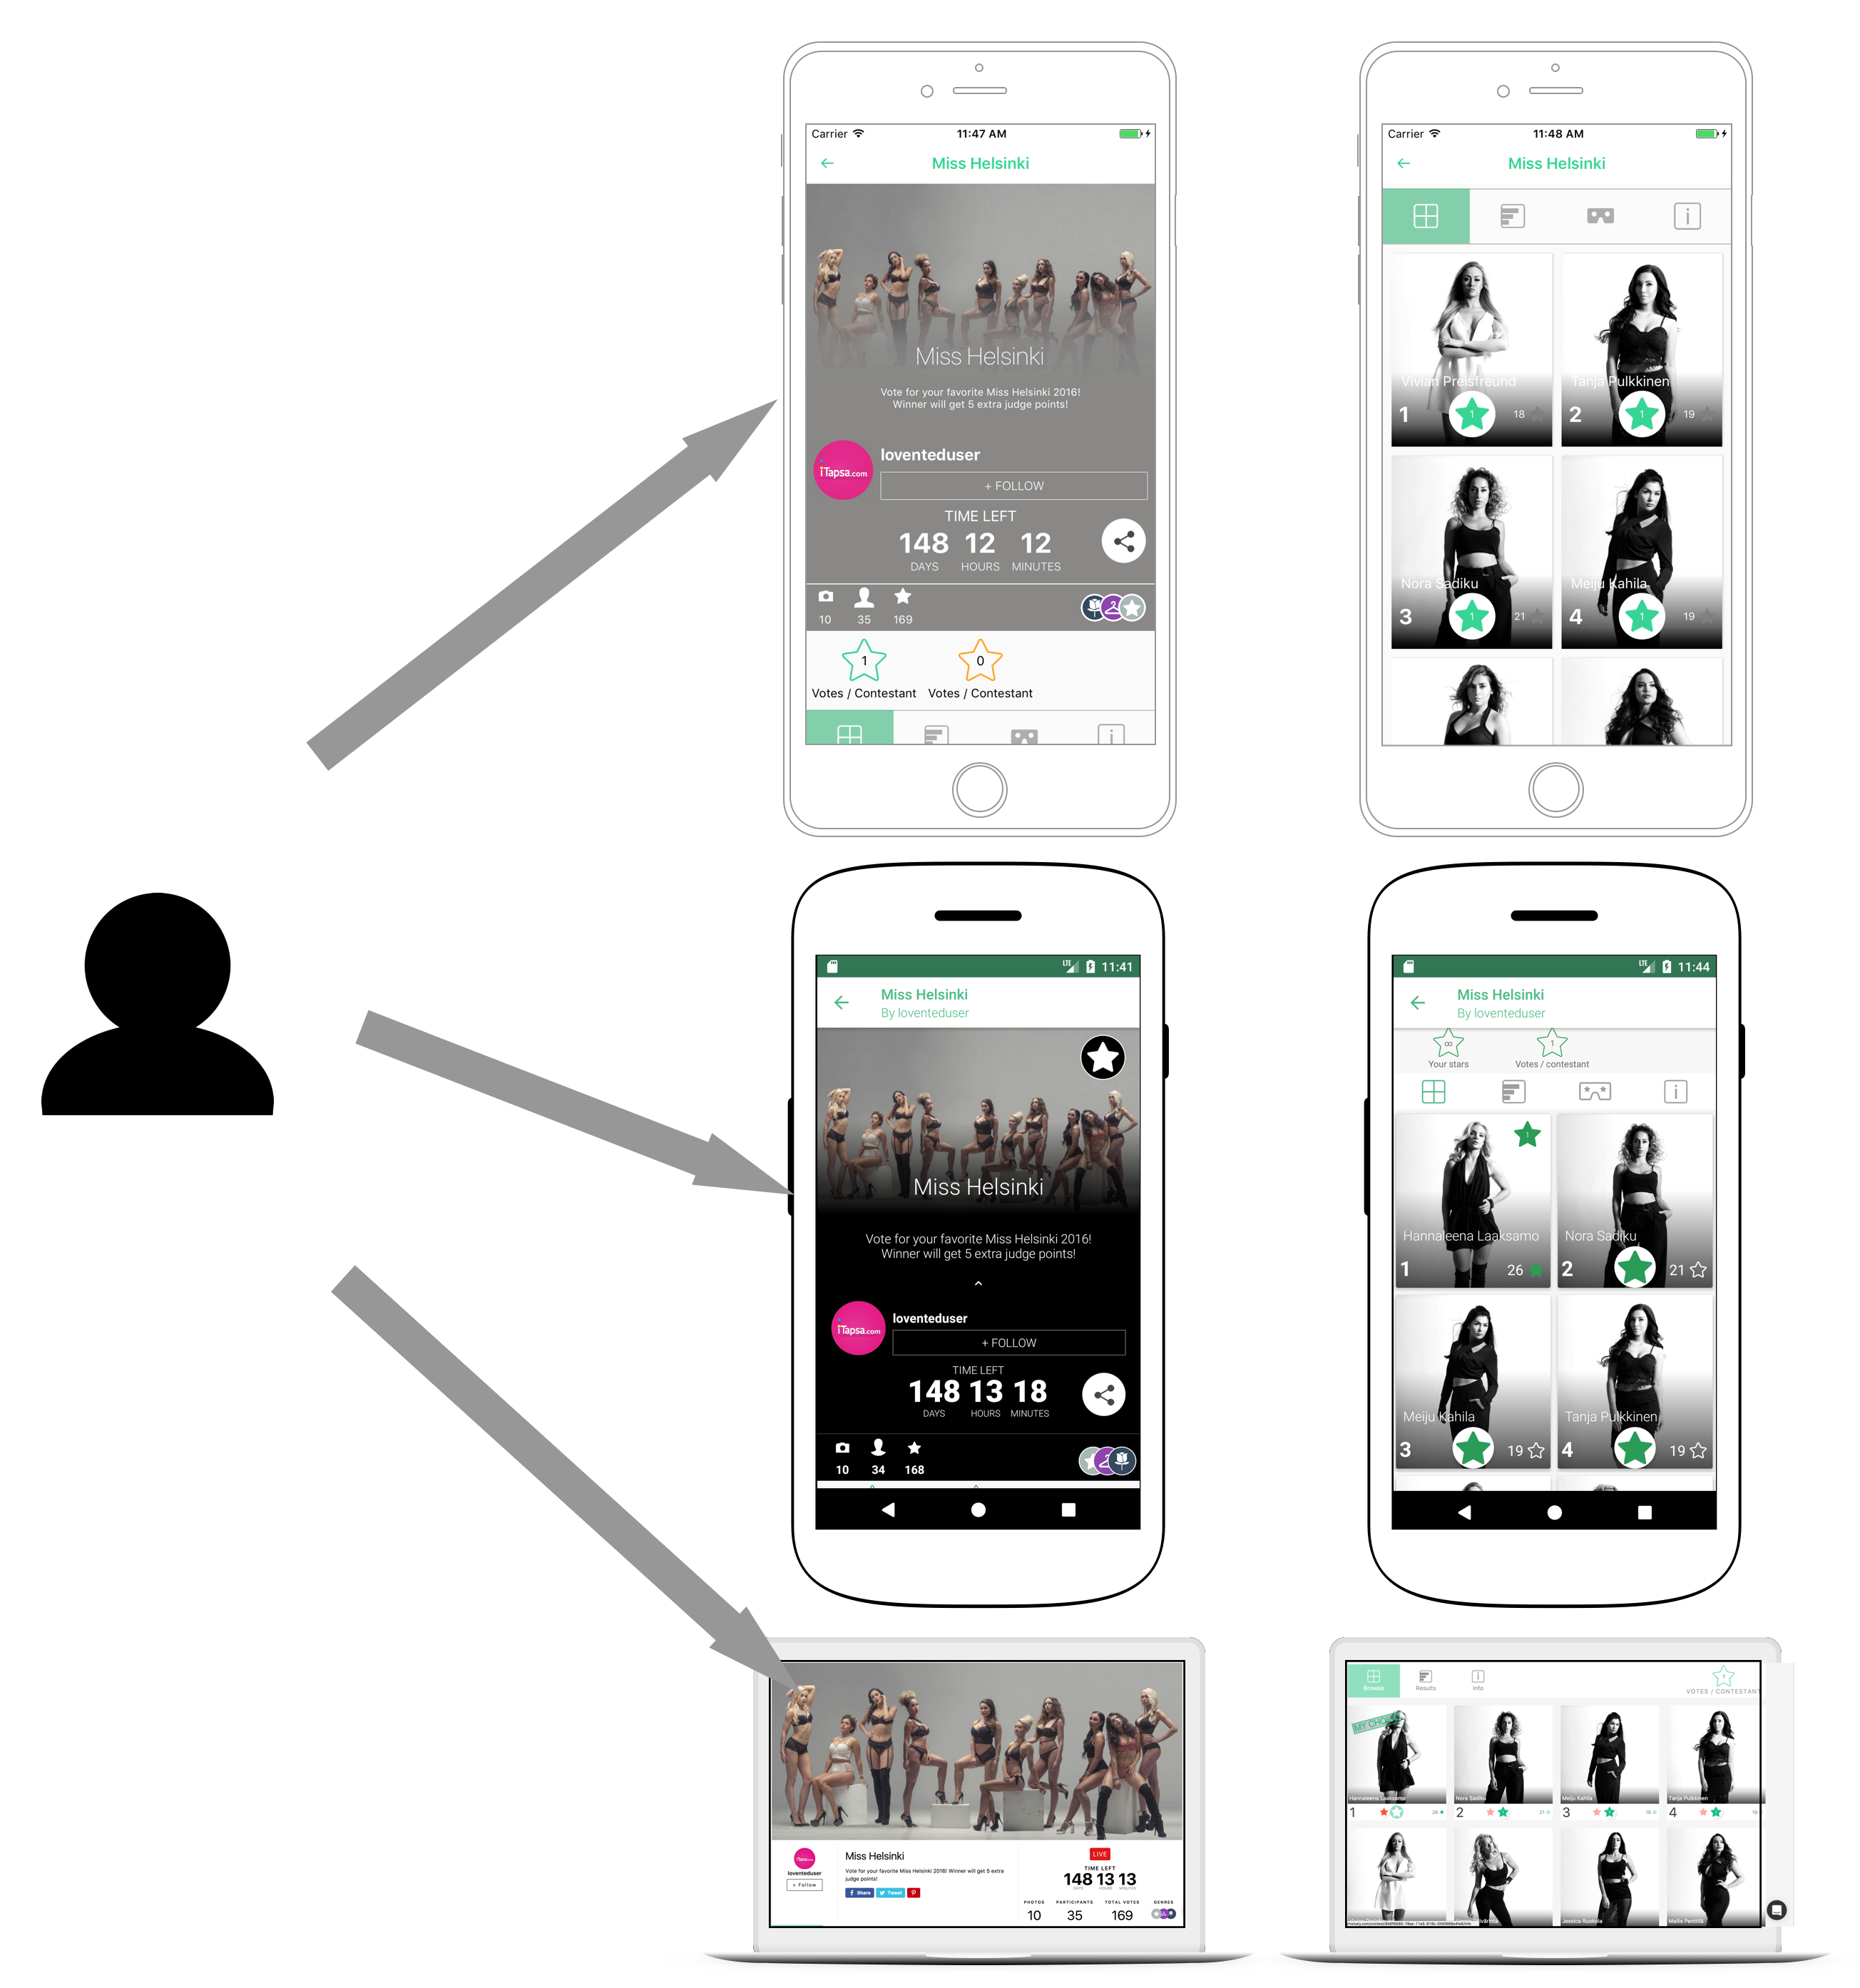
\includegraphics[width=0.6\textwidth]{images/choicely_platforms.png}
			\caption{Choicely collects data through three interfaces: iOS devices, Android devices and web.}
			\label{choicely_platforms}
		\end{center}
	\end{figure}

    % what kind of data is generated?
    The available data is two-folded: each user has a user profile, which contains basic demographical information about the user (gender and location), while contests have a number of participants with arbitrary number of votes that the users have spent on them. Depending on the configuration of contests, users may have limited number of votes to spend on every contest and participant, however there may be unlimited number of votes to spend on both. 

    % how does the data look like and how can it be retrieved?
    The data is structured in nature and is stored in a... The data can be accessed via...

    %  why is it important to analyze this kind of data and what can we learn from it? 
    There is a need to analyze this data, because...

    % why is the data analysis relevant from scientific research point of view?
    Performing scientific research on such data is interesting for multiple reasons...

\subsection{Research setting}
    % how computer vision is going to be utilized? 
    To model user behavior, computer vision is utilized in order to label the content of the images. Figure \ref{google_vision_labels} displays an example.  

    \begin{figure}[h] 
		\begin{center}
			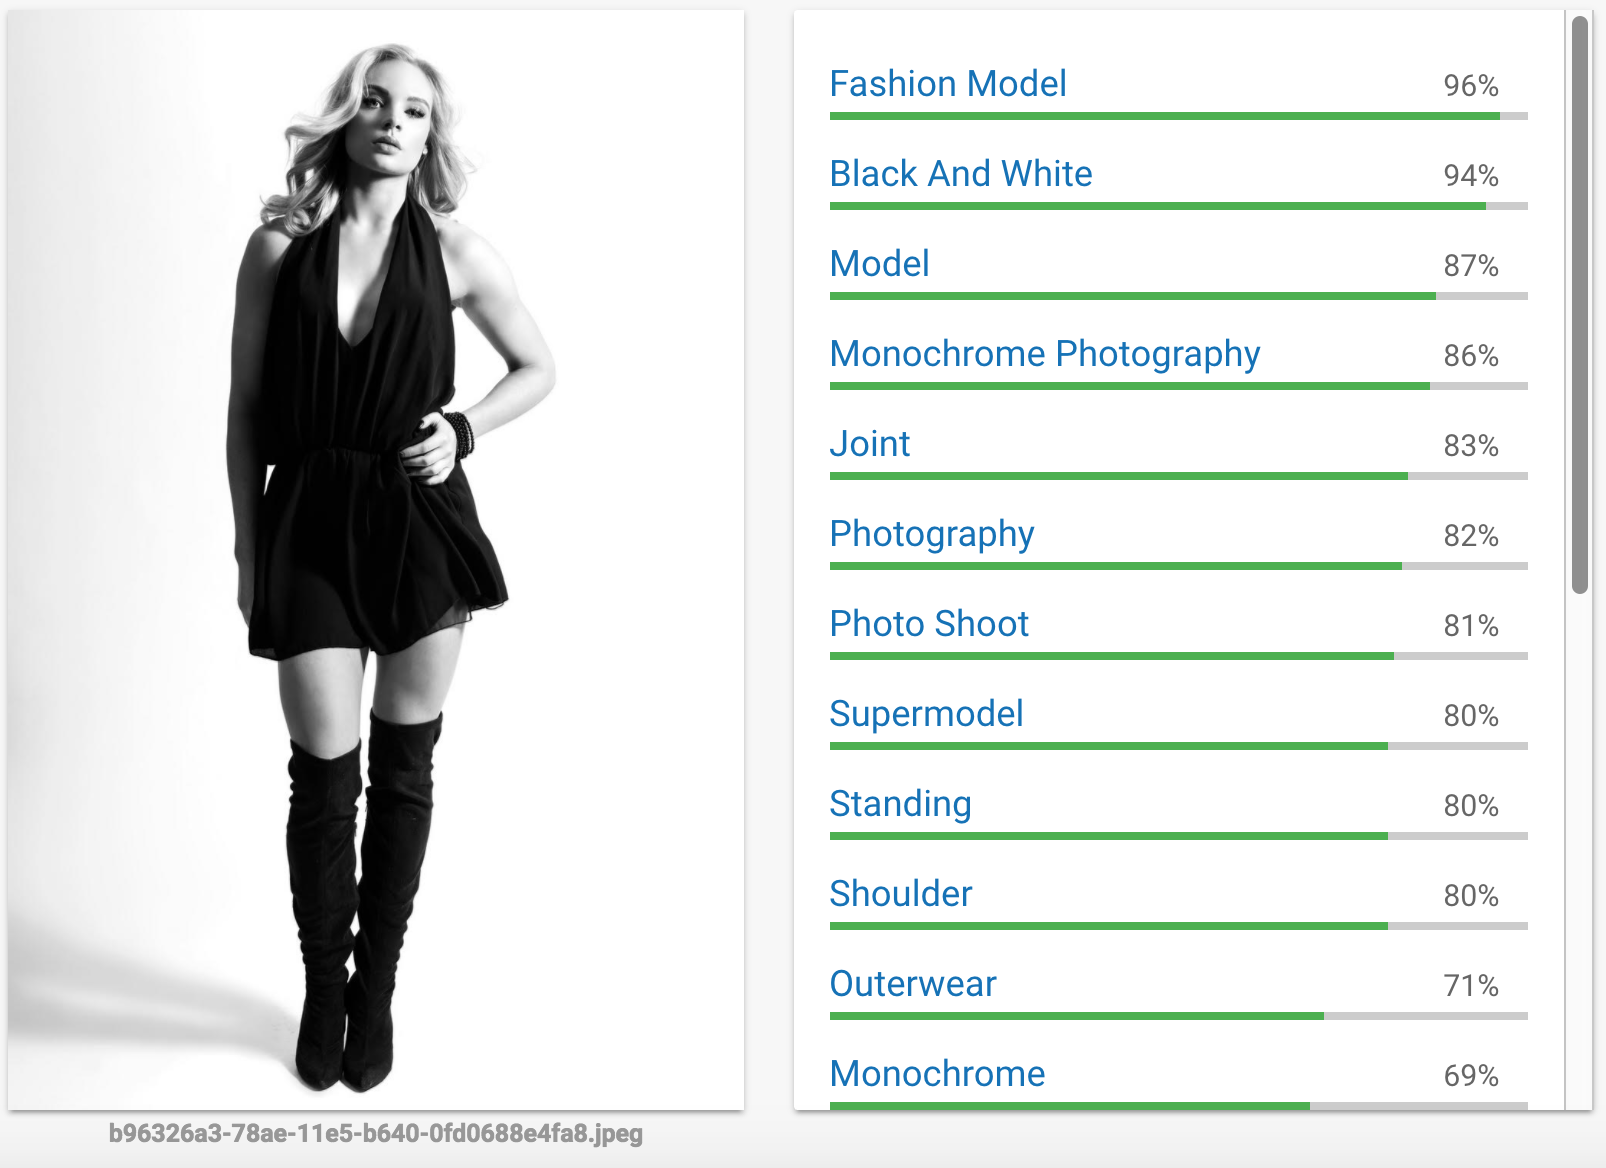
\includegraphics[width=0.6\textwidth]{images/google_vision_labels.png}
			\caption{The labels identified by the Google Vision API on one of the contest participant's image.}
			\label{google_vision_labels}
		\end{center}
	\end{figure}

\subsection{Methodology}
    % what kind of methods were chosen? 
    % what are the decisions behind the choices? 
    % what were the alternatives and why were they rejected? 

\subsection{Results}
    % what are the answers to RQ1? 
    % what are the answers to RQ2? 
    % what are the answers to RQ3?
    % what do the results mean? what are the implications? 